\documentclass[10pt, compress]{beamer}

\usetheme{metropolis}           % Use metropolis theme

\usepackage[export]{adjustbox}
\usepackage{booktabs}
\usepackage[scale=2]{ccicons}
\usefonttheme[onlymath]{serif}

%\usemintedstyle{trac}

\title{A review on methods for Bayesian hierarchical clustering}
\subtitle{}
\date{June 3, 2016}
\author{Sharad Vikram}
\institute{UCSD}

\setcounter{tocdepth}{1}

\begin{document}

\maketitle

\section{Background}

\subsection{Clustering}

\begin{frame}{Unsupervised learning}
  In unsupervised learning, we are interested in finding
        underlying structure
        in data.

  \pause
  Current methods include:
  \begin{itemize}
  \pause
    \item \textbf{Dimensionality reduction:} finding low-dimensional
      representations of high-dimensional data
  \pause
    \item \textbf{Clustering:} discovering natural groups
      in data
  \end{itemize}
\end{frame}

\begin{frame}{Clustering}
  The most popular methods for clustering produce
  flat clusterings.

  A \alert{flat clustering} is a partition of a set of data,
  or an assignment of each data point into one of
  several disjoint sets.
  
  \pause

  \begin{align}
    \{1, 2, \ldots, N\} \rightarrow \{\{\ldots\}, \{\ldots\}, \ldots, \{\ldots\}\}
  \end{align}
\end{frame}

\begin{frame}{Flat clustering}
  The most popular algorithm for flat clustering is \alert{k-means}.
  \begin{enumerate}
    \item<2-> Pick a number of clusters $K$.
    \item<3-> Randomly initialize cluster centers $\{\mu_1, \ldots, \mu_K\}$.
    \item<4-> Alternate until convergence:
      \begin{itemize}
        \item Assign each data point to its closest cluster center.
        \item Assign each cluster center to the mean of its assigned data points.
      \end{itemize}
  \end{enumerate}
  \uncover<5->{
  This is equivalent to optimizing the loss function:
  \begin{align}
    L(\mu_1, \ldots, \mu_K) = \sum_{i = 1}^N \min_k \|x_i - \mu_k\|^2_2
  \end{align}}
\end{frame}

\begin{frame}{Flat clustering: pros and cons}
  \begin{table}
    \begin{tabular}{lr}
      \toprule
      Pros & Cons \\
      \midrule
      Simple algorithms &  Requires specification of $k$ (in general)\\
      Efficient algorithms & \\
      Theoretical understanding & \\
      \bottomrule
    \end{tabular}
  \end{table}
\end{frame}

\begin{frame}{Hierarchical clustering}
  In \alert{hierarchical clustering}, data
  is recursively partitioned to form a tree (typically binary),
  also called a hierarchy.

  \begin{center}
    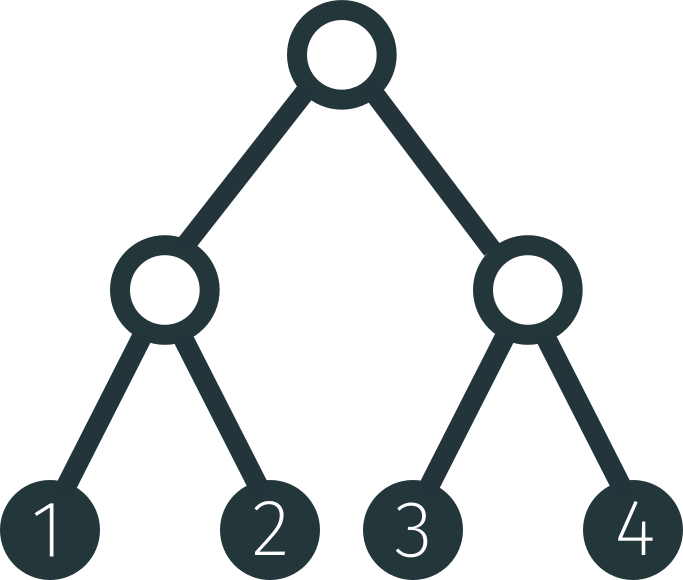
\includegraphics[width=0.5\textwidth]{img/tree-1234-balanced}
  \end{center}

  \pause

  Each leaf in the tree is a single data point,
  The root is the grouping of all data points
  into a single cluster and internal nodes
  are groupings of different granularities.
\end{frame}

\begin{frame}{Traditional hierarchical clustering algorithms}
  Hierarchical clustering algorithms can be broadly broken
  down into two categories:

  \begin{itemize}
    \item<2-> \textbf{Agglomerative (bottom-up):} the tree is built by
      beginning with just singleton clusters (leaves) and
      iteratively merging them until we have one cluster (root)
    \item<3-> \textbf{Divisive (top-down):} the tree is built
      by beginning with a single cluster (root) and
      recursively partitioning it until we
      have just singleton clusters (leaves)
  \end{itemize}
\end{frame}

\begin{frame}{Agglomerative clustering}
  The inputs to an agglomerative clustering algorithm
  are:
  \begin{itemize}
    \item<2-> Dataset $X = \{x_i\}_{i = 1}^N$
    \item<3-> Dissimilarity function $d(x, x')$
    \item<4-> Linkage criterion $D(A, B)$.
  \end{itemize}

\end{frame}

\begin{frame}{Dissimilarity functions}

  A dissimilarity function measures how
  different two data points are from each other.

  \pause

  Example dissimilarity functions include:
  \begin{itemize}
    \item Euclidean distance: $d(x, x') = \|x - x'\|_2^2$
    \item Manhattan distance: $d(x, x') = \|x - x'\|_1$
    \item Mahalanobis distance: $d(x, x') = (x - x')^T\Sigma(x - x')$
  \end{itemize}
\end{frame}

\begin{frame}{Linkage criteria}

  A linkage measures how
  different two \textbf{clusters} are from each other
  in terms of dissimilarity function $d$.

  \pause

  Example linkage criteria include:
  \begin{itemize}
    \item<2-> Single linkage: $D(A, B) = \min_{i \in A, j\in B} d(x_i, x_j)$
    \item<3-> Complete linkage: $D(A, B) = \max_{i \in A, j\in B} d(x_i, x_j)$
    \item<4-> Average linkage: $D(A, B) = \frac{1}{|A||B|}\sum_{i \in A, j\in B} d(x_i, x_j)$
  \end{itemize}
\end{frame}

\begin{frame}{Agglomerative clustering}
  We iteratively merge the two closest clusters until 
  we have one cluster left.

  \begin{center}
    \includegraphics<1>{img/agglomerative-clustering-0}
    \includegraphics<2>{img/agglomerative-clustering-1}
    \includegraphics<3>{img/agglomerative-clustering-2}
    \includegraphics<4>{img/agglomerative-clustering-3}

  \end{center}

  \centering
  \begin{itemize}
    \item<1>[] $\{\{1\}, \{2\}, \{3\}, \{4\}\}$\\
    \item<2>[] $\{\{1, 2\}, \{3\}, \{4\}\}$\\
    \item<3>[] $\{\{1, 2\}, \{3, 4\}\}$\\
    \item<4>[] $\{\{1, 2, 3, 4\}\}$\\
  \end{itemize}
\end{frame}

\begin{frame}{Agglomerative clustering examples}
  \begin{figure}
    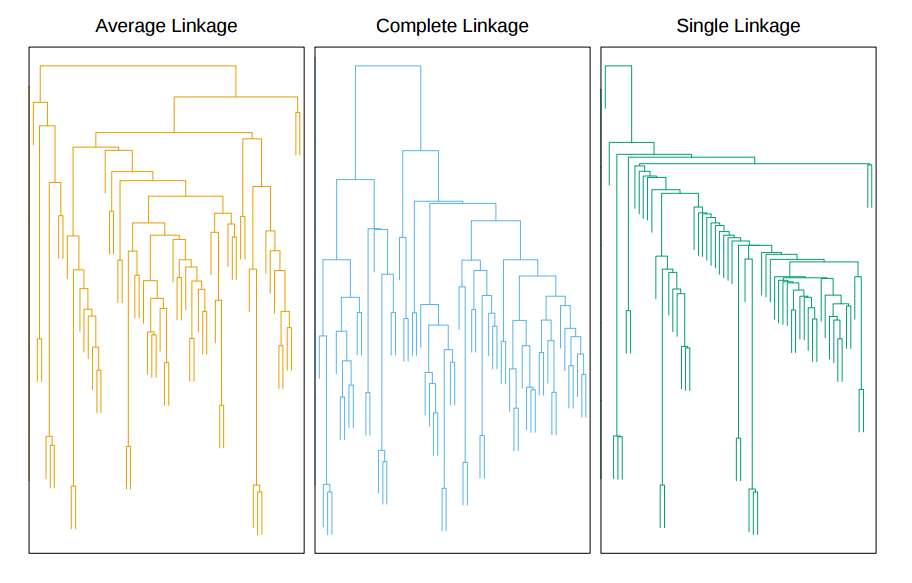
\includegraphics[frame,width=\textwidth]{img/dendrograms}
    \caption{Trees produced by agglomerative clustering algorithms
    with different linkage criteria. Source: \cite{Hastie2009}}
    \label{fig:dendrograms}
  \end{figure}
\end{frame}

\begin{frame}{Divisive clustering}
  In divisive clustering, we begin with the root cluster
  and recursively partition it until we are left with
  singleton leaf clusters.
\end{frame}

\begin{frame}{Ambiguous data}
  Consider the two following scenarios where
  circles represent tight clusters of data.

  \begin{center}
  \includegraphics[width=0.3\textwidth]{img/3-cluster}\hfill
  
\includegraphics[width=0.45\textwidth]{img/3-cluster-line}
  \end{center}

  \pause

  A single binary tree is not sufficient to describe either
  of these configurations.

  %\centering
  %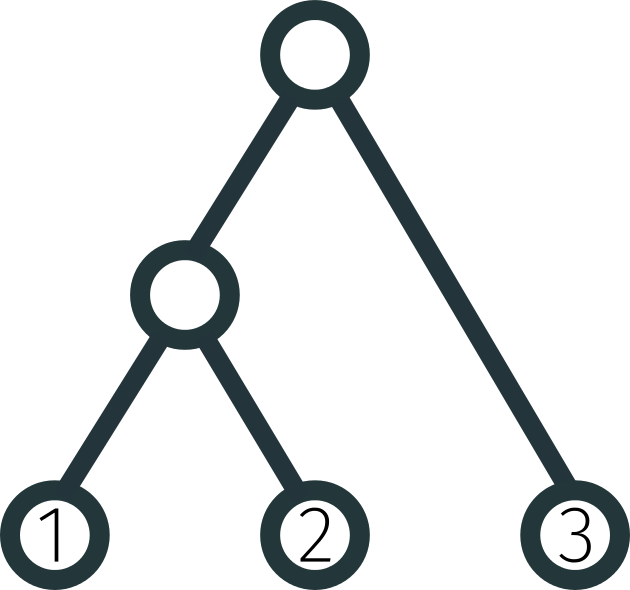
\includegraphics[width=0.3\textwidth]{img/tree-123} \hfill
  %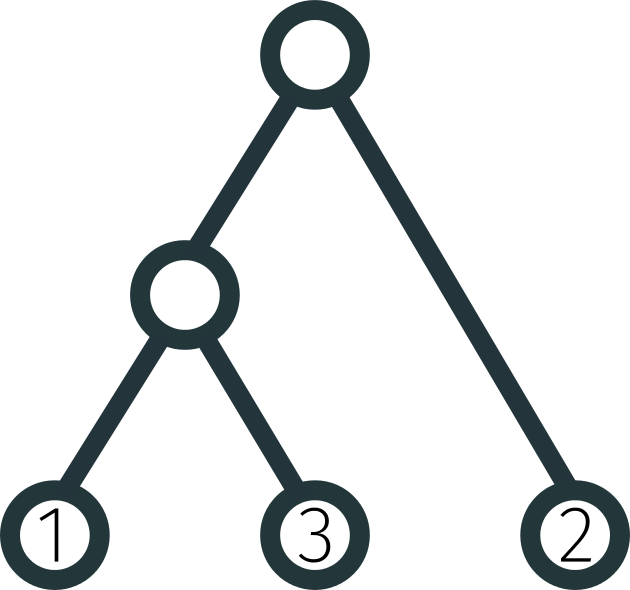
\includegraphics[width=0.3\textwidth]{img/tree-132} \hfill
  %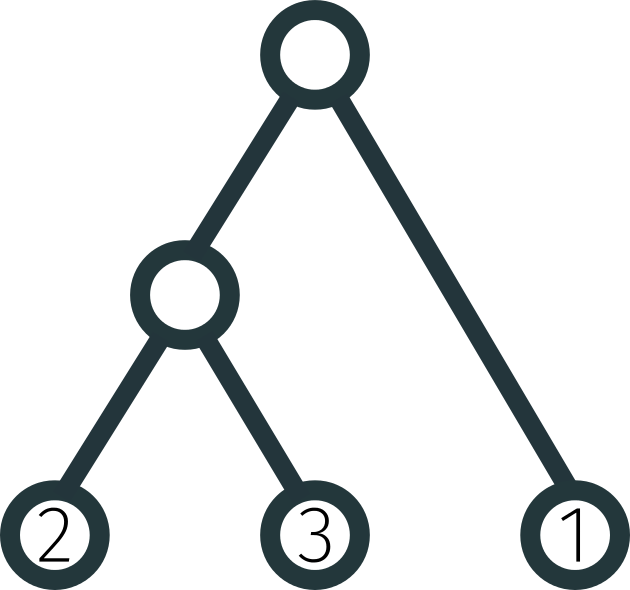
\includegraphics[width=0.3\textwidth]{img/tree-231}

\end{frame}

\begin{frame}{Multifurcating trees}
  Perhaps extending our binary trees to $k$-ary trees will help.

  \begin{center}
    \includegraphics<1>[width=0.8\textwidth]{img/3-cluster-both.png}
    \includegraphics<2>[width=0.8\textwidth]{img/3-cluster-both-2.png}
    \includegraphics<3>[width=0.8\textwidth]{img/3-cluster-both-3.png}
  \end{center}

\end{frame}

\begin{frame}{Uncertainty in hierarchies}
  Furthermore, small perturbations in our data
  can have an effect on the output
  hierarchy.

  \begin{center}
    \includegraphics<1>[width=0.8\textwidth]{img/3-cluster-line-noperturb}
    \includegraphics<2->[width=0.8\textwidth]{img/3-cluster-line-perturb}
  \end{center}

  \uncover<3>{We need a more general approach.}
\end{frame}

\begin{frame}{Probabilistic reasoning}
  A better approach is to
  model ambiguity and uncertainty with \textbf{probability}.
  Instead of outputting a single tree,
  we output a probability distribution over all possible
  trees.

  \begin{center}
    \includegraphics<2>[width=0.7\textwidth]{img/3-cluster-distribution.png}
    \includegraphics<3>[width=0.7\textwidth]{img/3-cluster-linear-distribution.png}
  \end{center}
\end{frame}

\subsection{Bayesian learning}

\begin{frame}{Latent variable models}
  We take a quick detour to review Bayesian learning.
  \begin{center}
    \includegraphics<2>[width=0.1\textwidth]{img/latent-variable-model-0}
    \includegraphics<3->[width=0.1\textwidth]{img/latent-variable-model}
  \end{center}
\uncover<4->{
  Our data $X$ is generated conditionally given a set of
  unobserved \alert{latent} variables $\theta$.
}
\end{frame}

\begin{frame}{Distributions of interest}
  We are interested in the \alert{posterior distribution}
  of latent variables given data, $P(\theta | X)$,
  calculated via Bayes rule.
  \pause

  \begin{align}
    P(\theta | X) = \frac{P(X | \theta)P(\theta)}{P(X)} = \frac{P(X | \theta)P(\theta)}{\int_\Theta P(X|\theta)P(\theta)d\theta}
  \end{align}
  \pause
  $P(\theta)$ is called the \alert{prior distribution} and $P(X|\theta)$ is called the
  \alert{likelihood model}. They are specified beforehand.
\end{frame}

\begin{frame}{Bayesian inference}
  Typically the hardest part of computing the
  the posterior distribution is calculating
  $P(X) = \int_\Theta P(X|\theta)P(\theta)d\theta$, the \alert{marginal distribution}.

   \pause 

  When the prior $P(\theta)$ and likelihood $P(X|\theta)$ are
  conjugate, the posterior is analytically computable.

  \pause

  Otherwise, we usually approximate it with methods such as:
  \begin{itemize}
    \item Loopy belief propagation
    \item Markov chain Monte Carlo (MCMC)
    \item Variational inference
    \item MAP estimation via EM
  \end{itemize}
\end{frame}

\section{Bayesian hierarchical clustering}

\begin{frame}{BHC as a latent variable model}
  Bayesian hierarchical clustering is a
  statistical approach, specifically
  a \alert{latent variable model}.
  \pause
  \begin{center}
    \includegraphics[width=0.3\textwidth]{img/bhc-lvm}
  \end{center}
  It is composed of data $X$ and
  latent variables $T$ and $\theta$.
  \pause
  \begin{itemize}
    \item $T$ is a tree structure, sampled from a \alert{tree prior} distribution $P(T)$.
    \item $\theta$ is a set of parameters, generated in a \alert{tree likelihood} model $P(\theta | T)$.
  \end{itemize}
\end{frame}

\begin{frame}{Tree priors}
  Most often we are interested in rooted binary trees with labeled leaves,
  also called \alert{cladograms}.

  \begin{center}
    \includegraphics<1>[width=0.4\textwidth]{img/tree-4}
    \includegraphics<2>[width=0.4\textwidth]{img/tree-4-ordering}
    \includegraphics<3>[width=0.4\textwidth]{img/tree-4-ordering-times}
  \end{center}

  Very often, cladograms will contain additional information.

  \begin{itemize}
    \item<2-> An ordering on the internal nodes
    \item<3-> Times associated with each node
  \end{itemize}

\end{frame}

\begin{frame}{Tree priors}
  Tree priors are probability distributions over cladograms
  and often include additional information
  in the nodes.

  \pause

  The simplest distribution is the uniform distribution over
  cladograms.

  \pause

  \begin{center}
    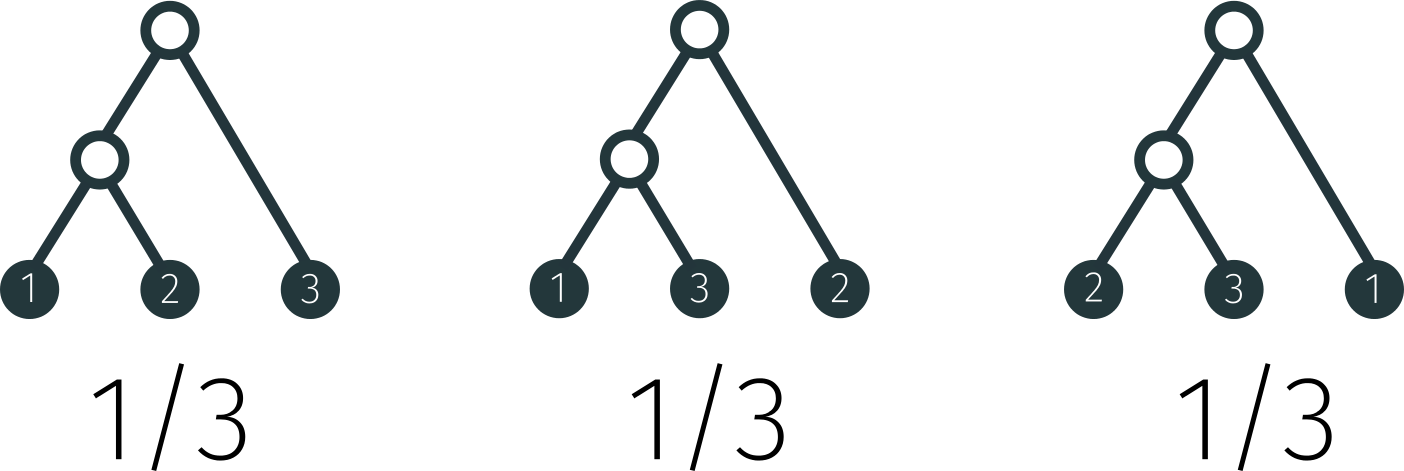
\includegraphics[width=0.6\textwidth]{img/uniform-distribution}
  \end{center}

  \pause
  In general, however, tree priors fall into two categories:
  \begin{itemize}
    \item \textbf{Coalescent models:} trees are modeled in a 
      agglomerative fashion, merging clusters until 
      one is left
    \item \textbf{Diffusion models:} trees are modeled inductively,
      starting with a tree of size $1$ and growing it to
      a tree of size $N$
  \end{itemize}
\end{frame}

\subsection{Coalescent models}

\begin{frame}{Coalescent models}
  Coalescent models begin with a set of $N$
  data, or "individuals", at $t = 0$.

  \begin{center}
    \includegraphics<1>[width=0.5\textwidth]{img/coalescent-1}
    \includegraphics<2>[width=0.5\textwidth]{img/coalescent-2}
    \includegraphics<3>[width=0.5\textwidth]{img/coalescent-3}
    \includegraphics<4>[width=0.5\textwidth]{img/coalescent-4}
  \end{center}

  \pause

  Every iteration, we:
  \begin{itemize}
    \item Pick two distinct nodes $a$ and $b$ uniformly at random.
    \item Sample a coalesce time $t$.
    \item Create an internal node whose children are $a$ and $b$
      with time $t$.
  \end{itemize}
\end{frame}


\begin{frame}{Kingman's coalescent}
  Coalescent models vary based on how times are sampled
  for internal node.
  The simplest coalescent model is \alert{Kingman's coalescent} \cite{Kingman1982},
  where we assume a constant coalesce rate.

  \pause

  Let $\delta_i$ represent the elapsed time
  between coalescent event $i-1$ and $i$.
  We let
  \begin{align}
    \delta_i \sim Exp\left(\binom{N - i + 1}{2}\right)
  \end{align}
\end{frame}
\subsection{Diffusion models}
\subsection{Other models}
\subsection{Generalizations}
\subsection{Inference}

\section{Adding interaction}

\subsection{Hierarchical clustering with constraints}
\subsection{Intelligent subset queries}

\section{Conclusion}

\begin{frame}[standout]
Questions?
\end{frame}

\begin{frame}[allowframebreaks]{References}
  \bibliography{main}
  \bibliographystyle{unsrt}
\end{frame}

\end{document}
